%%%%%%%%%%%%%%%%%%%%%%%%%%%%%%%%%%%%%%%%%
% a0poster Landscape Poster
% LaTeX Template
% Version 1.0 (22/06/13)
%
% The a0poster class was created by:
% Gerlinde Kettl and Matthias Weiser (tex@kettl.de)


\documentclass[11pt,twoside,a4paper]{article}

\usepackage{multicol} % This is so we can have multiple columns of text side-by-side
\columnsep=100pt % This is the amount of white space between the columns in the poster
\columnseprule=3pt % This is the thickness of the black line between the columns in the poster

\usepackage[svgnames]{xcolor} % Specify colors by their 'svgnames', for a full list of all colors available see here: http://www.latextemplates.com/svgnames-colors

\usepackage{times} % Use the times font
%\usepackage{palatino} % Uncomment to use the Palatino font

\usepackage{graphicx} % Required for including images
% Location of the graphics files

\graphicspath{
{Graphics/}
}

\usepackage{url}
\usepackage{booktabs} % Top and bottom rules for table
\usepackage[font=small,labelfont=bf]{caption} % Required for specifying captions to tables and figures
\usepackage{amsfonts, amsmath, amsthm, amssymb} % For math fonts, symbols and environments
\usepackage{wrapfig} % Allows wrapping text around tables and figures


 %%% About citations presentation 
\usepackage[comma,authoryear]{natbib}
% Redefining \cite as \citep 
\let\oldcite\cite
\renewcommand{\cite}{\citep}

%% FOR IAOS: 
%\usepackage[numbers]{natbib}  %   <----- This for IAOS 

\definecolor{vert}{rgb}{0.1,0.7,0.2}
\definecolor{brique}{rgb}{0.7,0.16,0.16}
\definecolor{gris}{rgb}{0.7, 0.75, 0.71}
\definecolor{twitterblue}{rgb}{0, 0.42, 0.58}
\definecolor{airforceblue}{rgb}{0.36, 0.54, 0.66}

\begin{document}

\begin{center}
\color{NavyBlue} \textbf{How [Not] To Lie with Graphics} \color{Black}\\ % Title
\textit{A Practitioner's Guide for Official Statistics}\\[1cm] % Subtitle


 \textbf{Christophe Bontemps}\\ % Author(s)
 Statistical Institute for Asia and the Pacific\\ % University/organization

\texttt{Christophe.Bontemps@un.org}\\ % Email address

%
\includegraphics[width=20cm]{SIAP_logo_2020_1800.png} % Logo or a photo of you, adjust its dimensions here

\end{center}

\vspace{0.1cm} % A bit of extra whitespace between the header and poster content


\begin{abstract}

\emph{Data visualization is one of the key elements to inform a wide range of statistics consumers, from medias to politicians and obviously,  the general public. In this field of communication,  NSOs who are in competition with other public and private communication channels, must differentiate themselves by the quality, accuracy and efficiency of the information they release, in particular through statistically-based graphics and graphical interfaces. But as for any statistics, data visualization should be designed to help the understanding of complex phenomena and  facilitate fair comparisons. They must act as visual statistical tests  and reveal unambiguous patterns and data-based “truths”. This paper propose to highlighting commonly encountered “visual lies”, that is data visualizations where what is represented (or perceived) is not what is present in the data set. Such representations can alter the perception of the underlying statistical messages and values delivered to various users and medias. Our approach is based on 10 rules that can be used to drastically change the understanding of the information represented from any given data set. We preach here counterexamples to reveal the best practices, in an attempt to promote data visualizations as a powerful tool for trustworthy communication of Official Statistics.}
\end{abstract}


\section{Introduction}
In a world saturated with data and competing narratives, the role of National Statistical Offices (NSOs) as trusted providers of accurate and impartial information is more vital than ever \cite{Hossein2023-DataGov}, \cite{Schreyer2024-Intw}, \cite{Perucci22024-Trust}, \cite{Pullinger2020-Trust}. Increasingly, and since the early hours of the Covid-19 pandemic, data visualization has emerged as a critical and powerful medium for public communication of statistical indicators and data-based analysis. When thoughtfully designed, graphical representations enable users, \emph{ e.g.}  policymakers, journalists, or general public, to grasp complex trends, identify disparities, and draw data-based conclusions. However, as with all forms of statistical communication, graphics carry choices that can enhance or undermine the credibility of the information they are meant to convey. This is well documented in statistics were statistical fallacies \cite{Huff1993} and paradoxes \cite{blyth1973simpson} are well-known and well taught in 101 statistical courses. 

Data visualization, however, remains an undervalued component of statistical practice, with traditional approaches often prioritizing modeling over communication \cite{Wickham2014}. While basic graphical tools are typically introduced for exploratory analysis, most mainstream statistical training overlooks the cognitive pitfalls and perceptual biases inherent in visual representation \cite{Cleveland1984}, \cite{Cairo2019} \cite{healey2007perception}.


%While most NSOs adhere to principles of objectivity and professional standards, they face growing pressure to compete in a crowded information ecosystem. Social media, data journalism, and private think tanks all vie for public attention—often with more visually engaging or simplified messages. This environment risks incentivizing shortcuts in visual design that may sacrifice nuance, fairness, or even accuracy.

This paper critically examines how visual representations can inadvertently (or purposefully) mislead, drawing attention to what we call “visual lies”, a term defined by \cite{Tufte2001} as situations where the representation or the impression conveyed by a graphic does not match the underlying data. While the term "lie"  is deliberately provocative even if inspired by two seminal references in statistics \cite{Huff1993} and geospatial representation  \cite{Monmonier1991}, our aim is constructive: to expose common pitfalls in data visualization and offer best practices that reinforce the credibility and communicative power of official statistics.

While some authors rightfully claim that the choice of any graphical form shouldn't be dictated by rules \cite{Cairo2019}, but should be data, message and audience driven, we have opted here for ten core rules that highlight typical misrepresentation. Thus, we present here counterexamples to promote a more thoughtful use of graphics, departing from usual practices, habits and software defaults. By identifying the mechanisms through which visual distortion occurs and how it can be avoided, we hope to contribute to ongoing efforts within the statistical community to improve user engagement, statistical and visual literacy and ultimately trust in the dissemination of public data by NSOs.


\section{Data visualization}

Data visualization, broadly defined as the graphical representation of qualitative or quantitative data to enhance understanding and communication \cite{Cleveland1993Book}, serves both exploratory and explanatory purposes, helping analysts understand data and enabling audiences to grasp findings quickly and intuitively. Following \cite{buja2009}, we can also consider consider data visualization as a  tool for exploring data and  detecting (discovering) structural information in a given data set. This idea of data visualization as a visual statistical test is presented in  Figure \ref{fig:VisualTest} with an example of how a  simple scatterplot can act as a feature detection. More precisely, the generic visual test can be formalized as:\\
\begin{center}
  $H_0$ : \{There is "nothing"  \} = \{\textbf{No} feature, \textbf{No} discovery\} \\
 \emph{vs}\\
  $H_1$ : \{ There is "something" \} = \{There is \textbf{``some''} feature \}
\end{center}

The implicit null hypothesis $H_0$ tested can obviously vary with the type of graphic and the data set under scrutiny, but there is a parallelism between quantitative testing and visual testing, or first step discovery. 

\begin{figure}[tbh]
\begin{center}
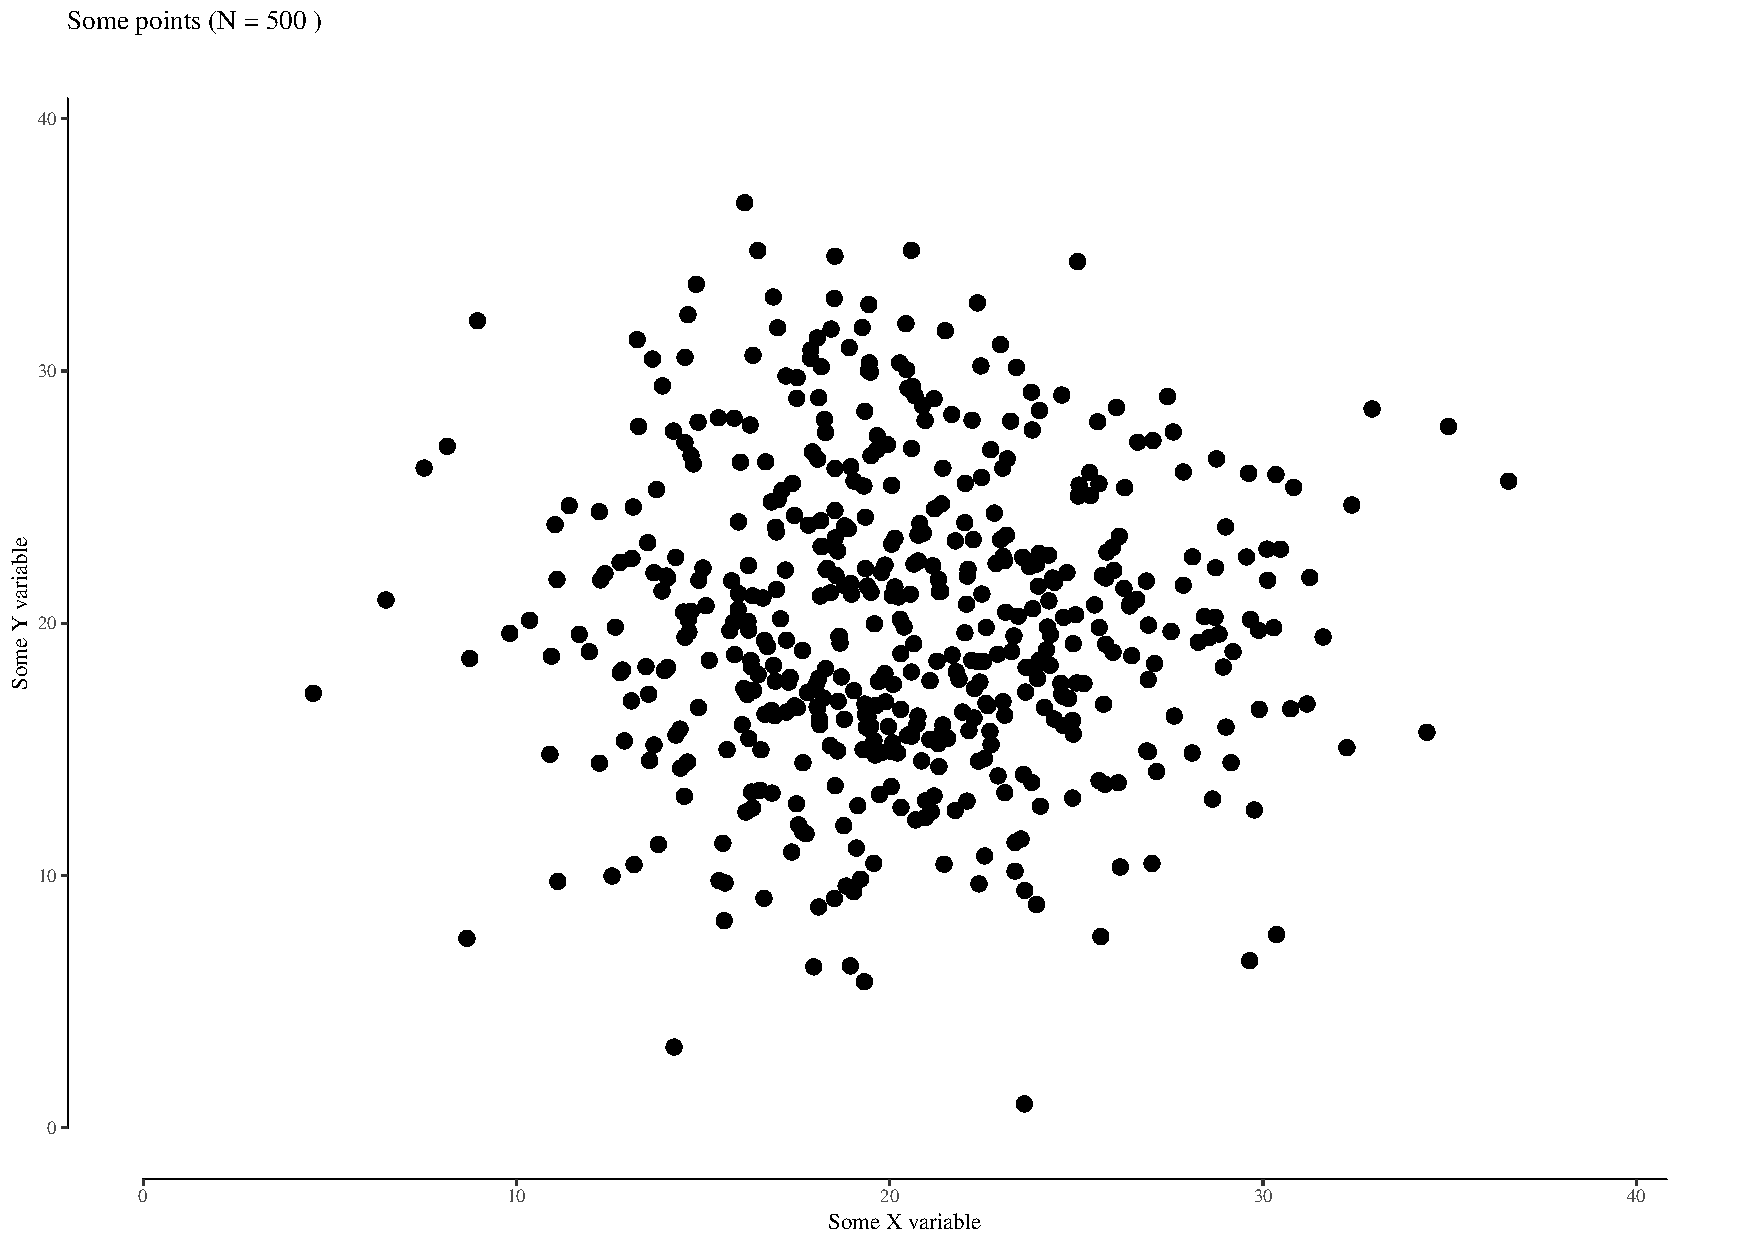
\includegraphics[width = 0.22\linewidth]{RandomPoints.pdf}
            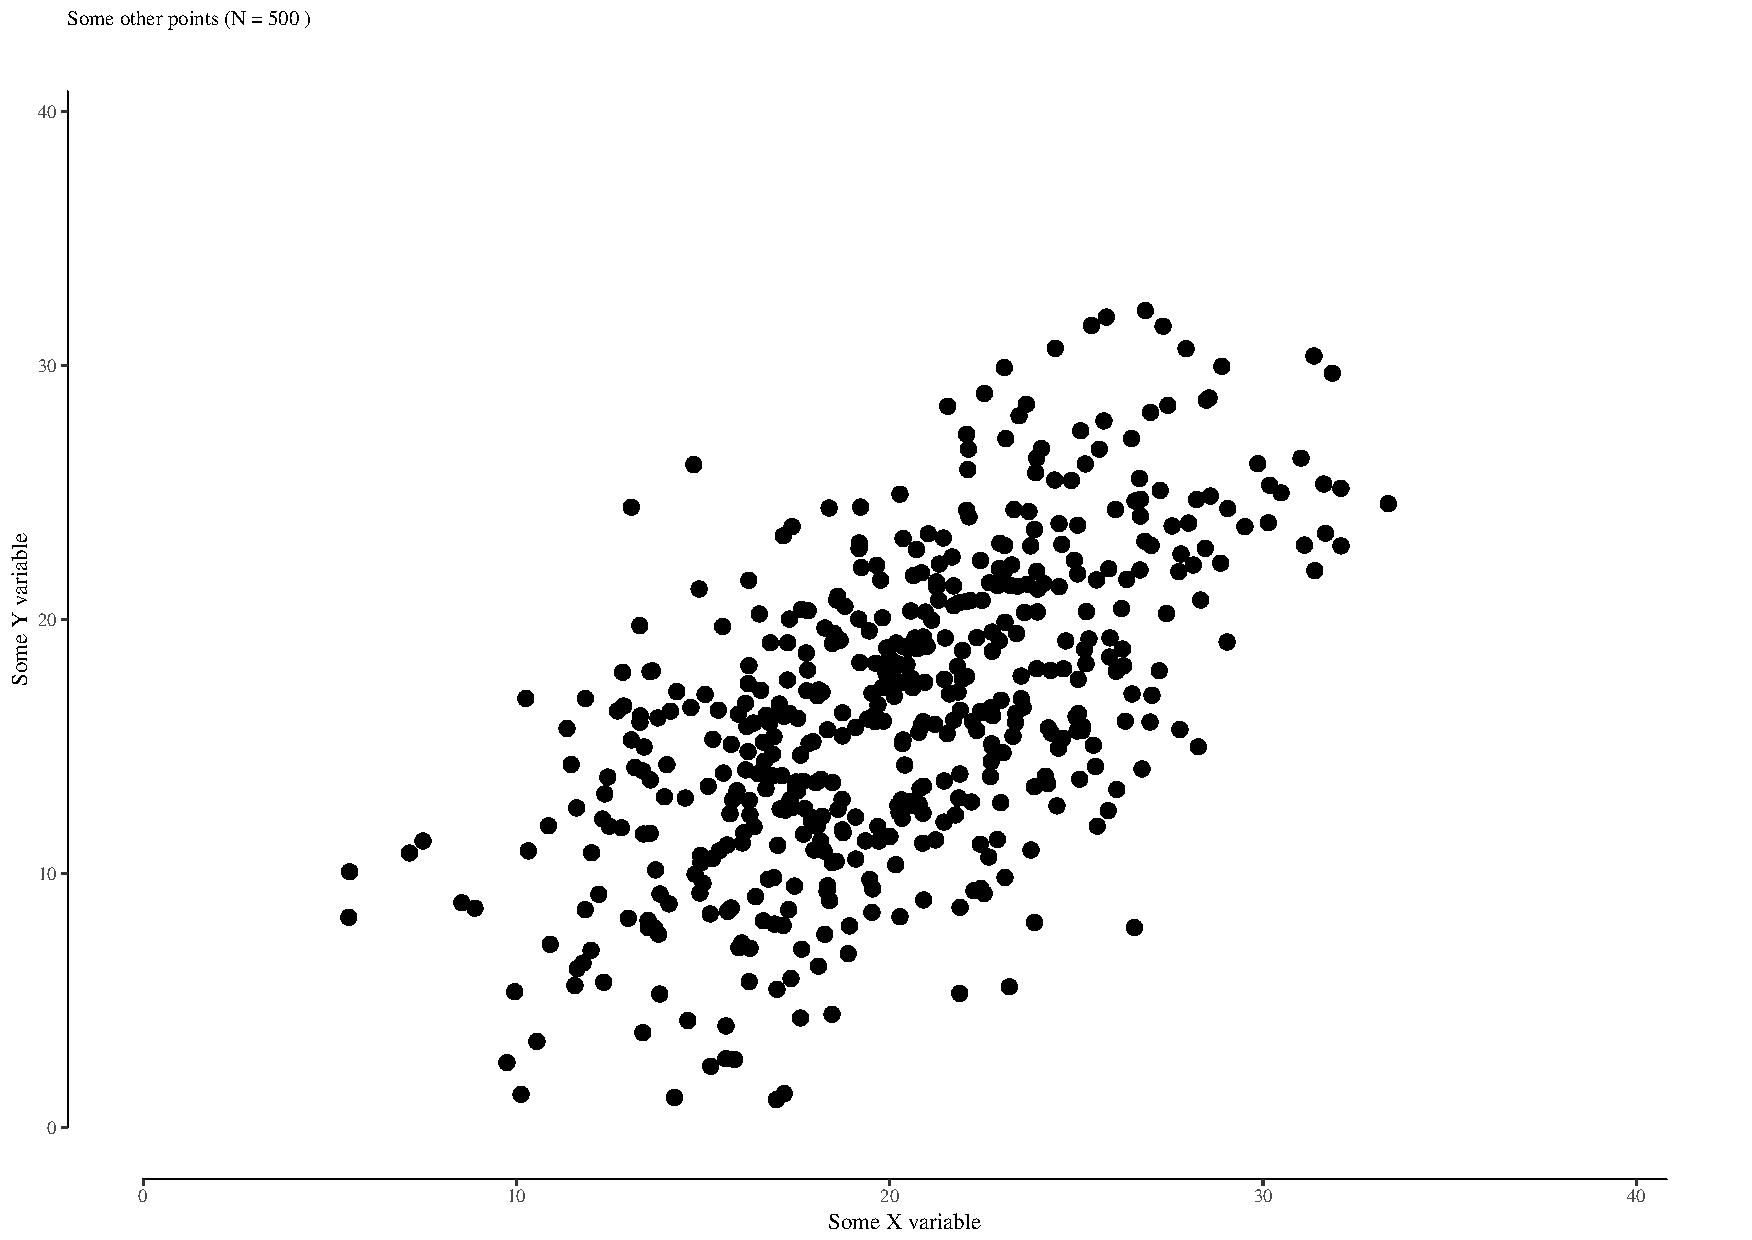
\includegraphics[width = 0.22\linewidth]{LinearPoints1.pdf}
            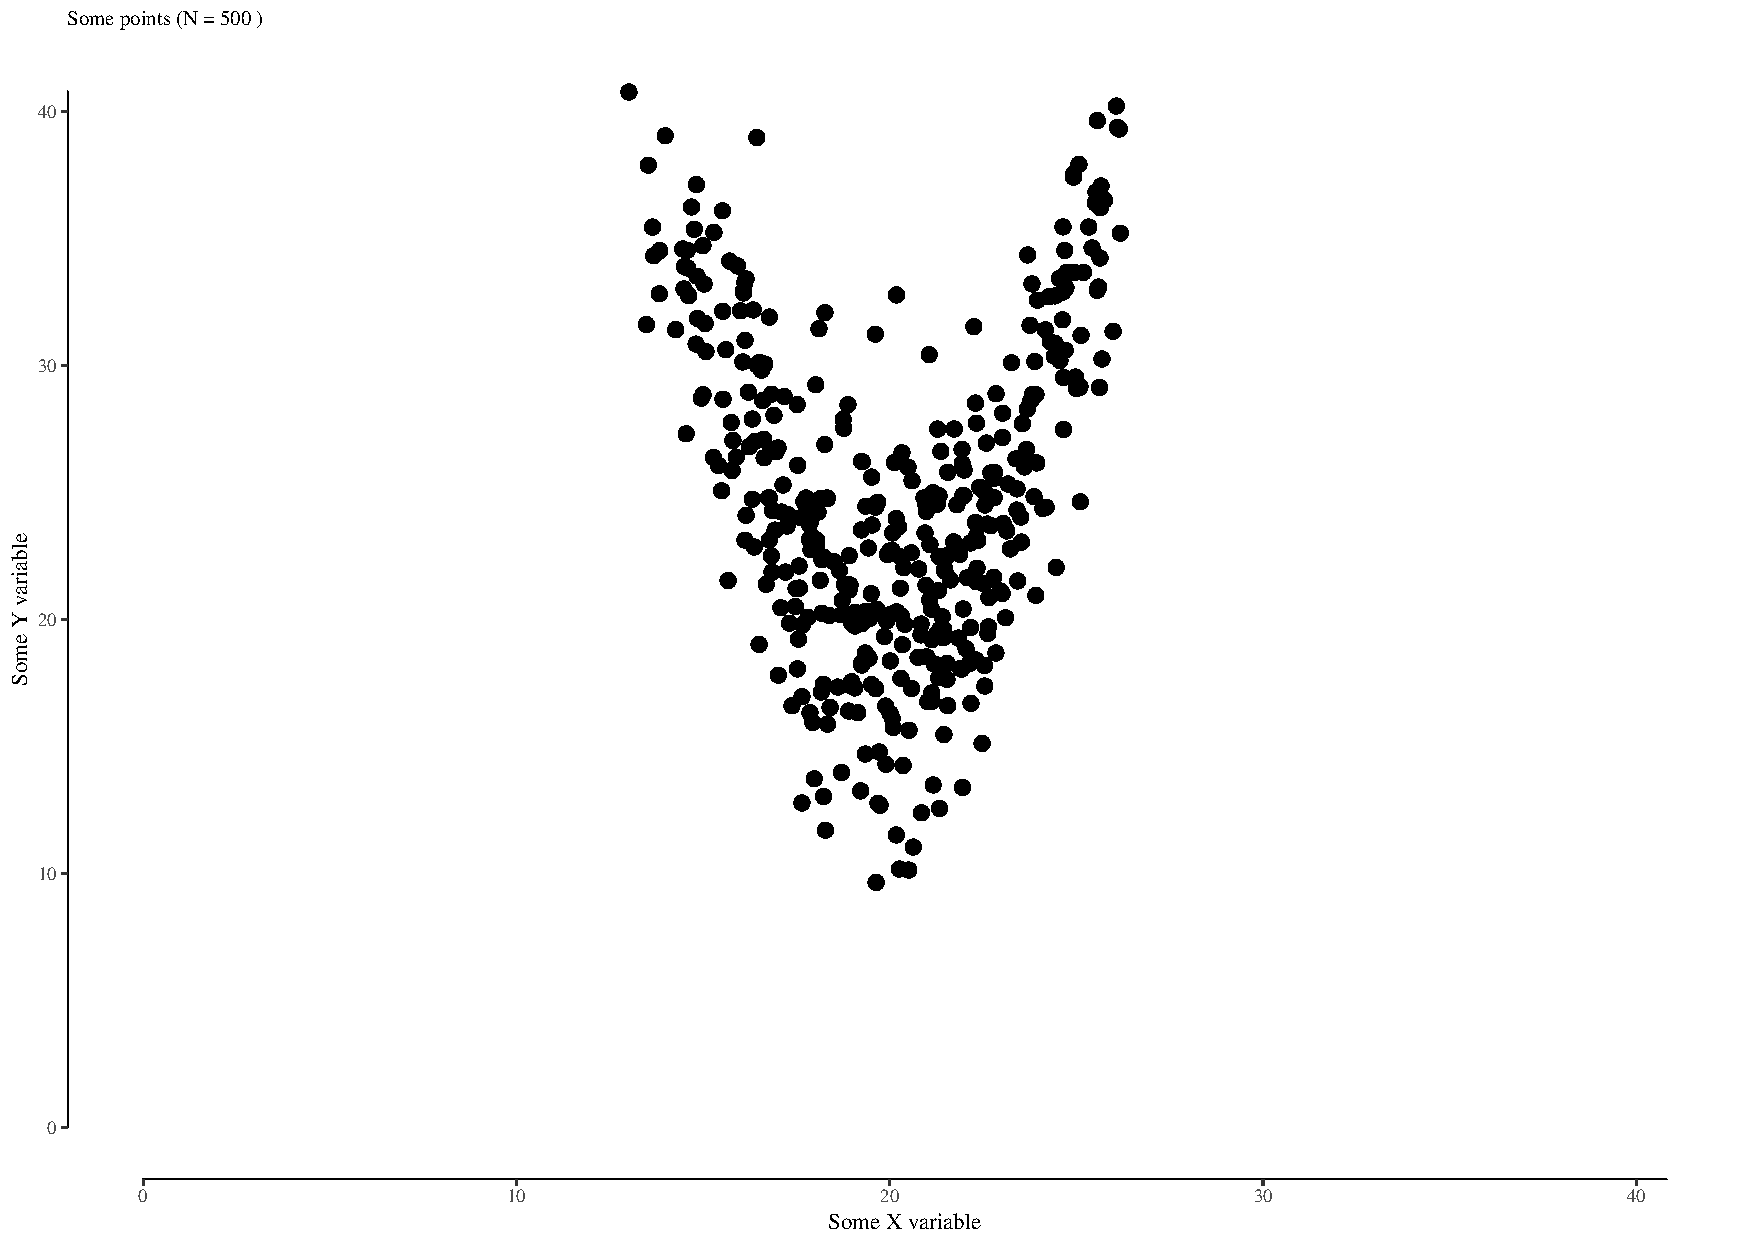
\includegraphics[width = 0.22\linewidth]{UshapedPoints.pdf}
            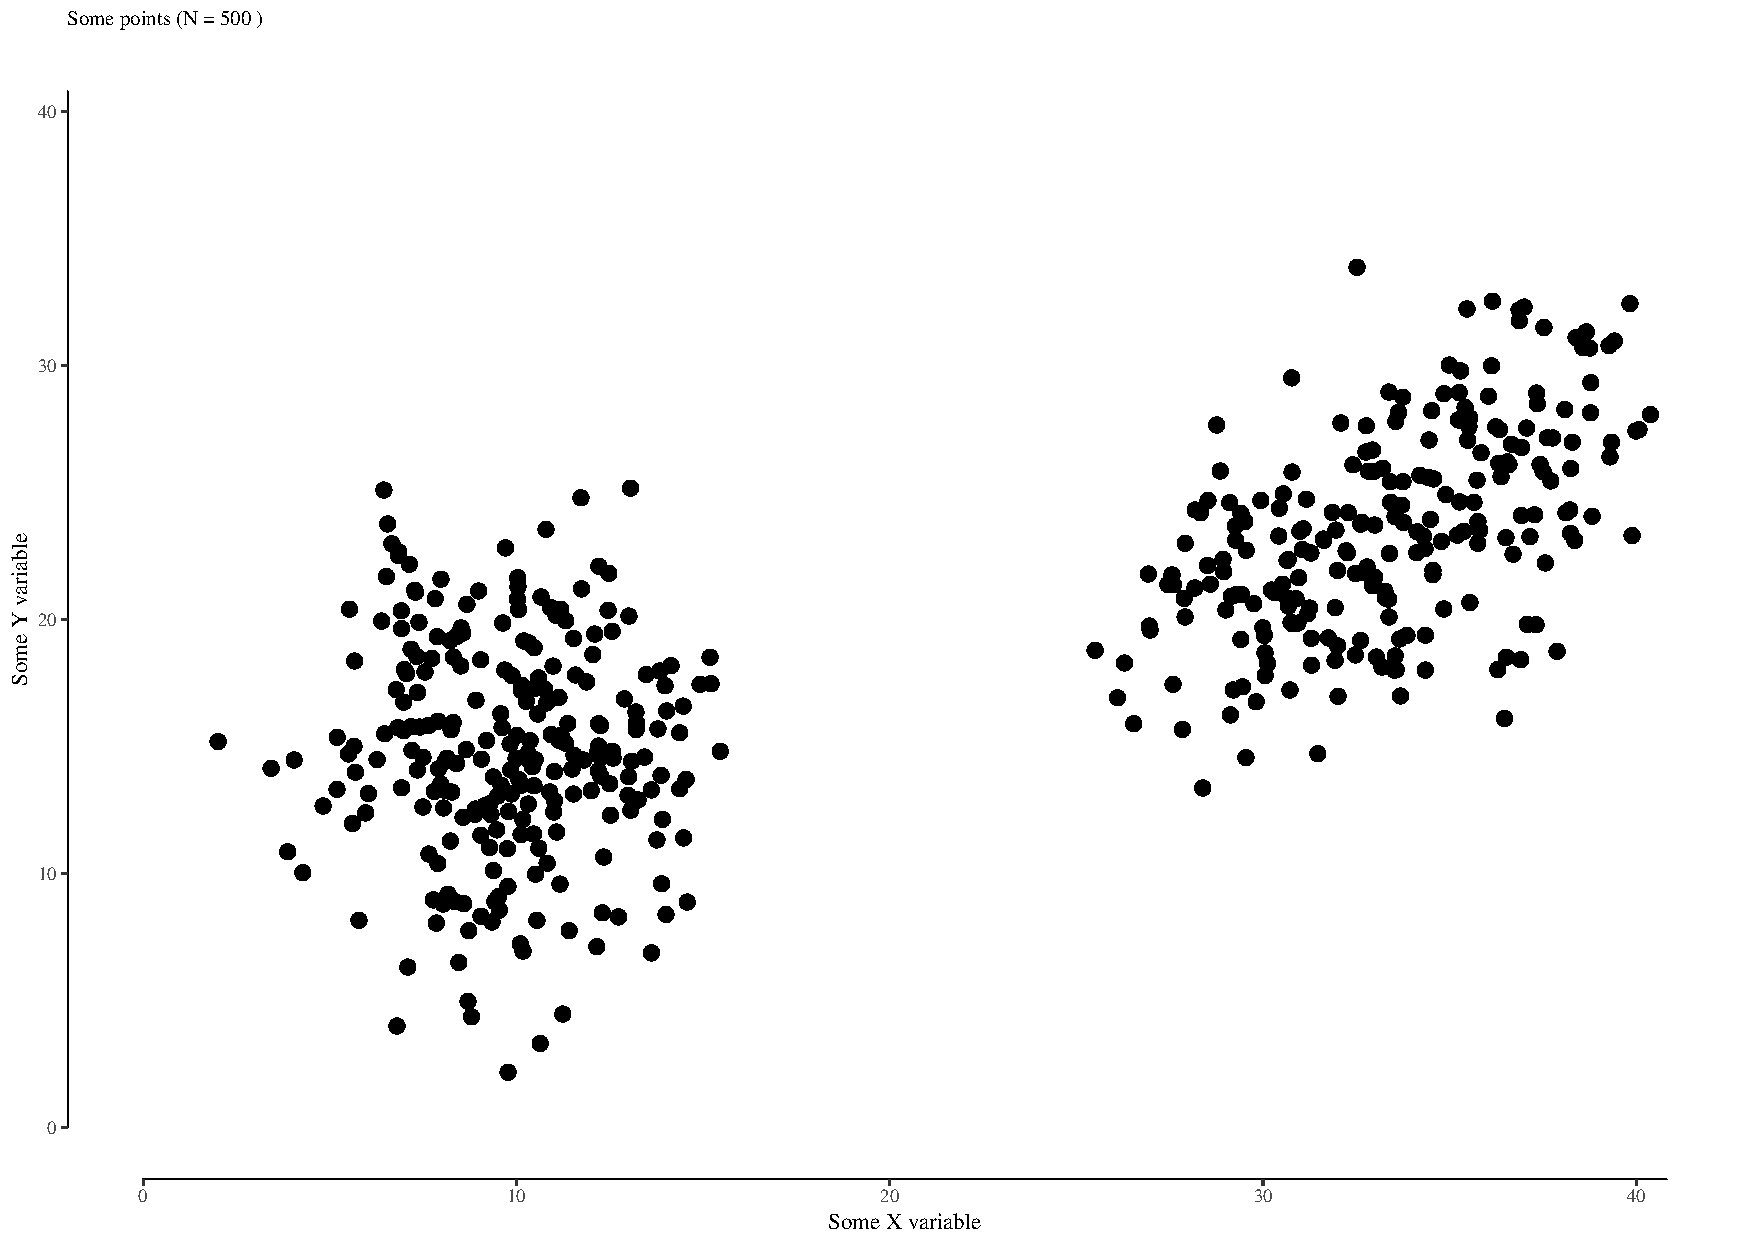
\includegraphics[width = 0.22\linewidth]{GroupsPoints.pdf}

\caption{Simple scatter plot can serve as a visual test. Only in the left hand-side plot $H_0$ is \textbf{not} rejected ("nothing" detected). In all three others, there is a feature (correlation, U-Shape, two groups) detected. }
%- "\emph{There's nothing}" (plot \#1), $H_0$ rejected - "\emph{There's a trend}" ( plot \#2), $H_0$  rejected - "\emph{There's a U-shaped relation}" (plot \#3), $H_0$ rejected - "\emph{There's groups}" (plot \#4)    }
\label{fig:VisualTest}
\end{center}
\end{figure}

When analysing and visualizing a data set, any data analysts or statistician implicitly performed this visual test. This is also what any viewer, not aware of the power of statistics, does when looking at any graphic. In his seminal book,  \cite{Bertin1983English}  has a more pragmatic approach stating that anyone should get right answers to legitimate questions when looking at any graphic provide that it well designed and accompanied with contextual information (caption, title, etc.)  
However, despite its simplicity and effectiveness, this test crucially relies on the good alinement of the visual representation with the feature under scrutiny and with  data set.  Moreover, as any statistical summary and 2-D object, it carries a risk of distortion due to a bad choice of the graphical form or visual encoding of the embedded information. The test may then fail due to a failure to comply with good practices leading to distortions of the information in the graphical representation.
 
 To measure the extend of this distortion \cite{Tufte2001} introduced the concept of the “\emph{lie factor}”, defined as the ratio of the effect shown in a graphic to the effect actually present in the data. 
 \begin{equation}
 \nonumber
\text{Lie Factor} = \frac{\text{Size of effect shown in graphic}}{\text{Size of effect in data}}
\end{equation}
 
 A lie factor far from 1.0 indicates a misrepresentation of the data, impeaching any valid visual test. 
  These risks are particularly consequential in the realm of official statistics, where public trust and informed decision-making depend on clarity, transparency, and fairness in communication.


 Institutional guidance from Eurostat \citep{Eurostat2022} and the OECD \citep{OECD2017} emphasizes the increasing importance of effective visualization in ensuring statistical messages are not only seen but also correctly interpreted.



 

%In this article, we call lie a situation where what is represented or perceived is not what is not present in the data set.

%----------------------------------------------------------------------------------------
%	Rules
%----------------------------------------------------------------------------------------


\section{Rule \#1: Modify Axes}

\textbf{CITE \cite{Xiong2021-VisuBar} here in conclusion to highlight the difficulty to use multiple bar charts for comparisons}

 \textbf{ ALSO \cite{correll_truncating_2019} on truncated axis}

One of the most common problem is the truncation of the vertical axe in bar charts, inducing an exaggerating effect.
\begin{center}
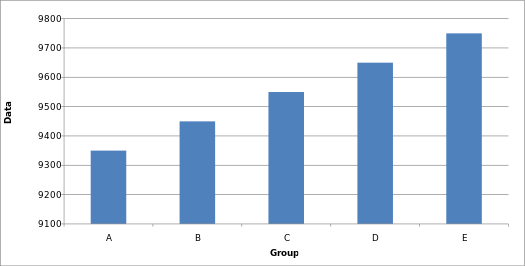
\includegraphics[width = 0.4\linewidth]{Truncated_Bar_Graph.png} 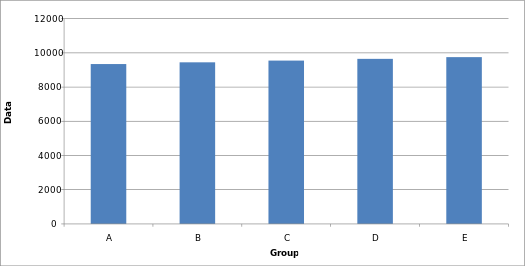
\includegraphics[width = 0.4\linewidth]{Bar_graph.png}
\captionof{figure}{\color{DarkSlateGray} {Truncation exaggerating effect (left), small absolute variation(right)}}
\end{center}

Interestingly,  \cite{Correll2019} experimentally showed that this exaggerating effect is also found in line charts (Figure 1b). This poses the question of when it is appropriate to start line chart at the origin, in particular when the origin is out of the range of the data set (ex: Earth temperature in Fahrenheit).
\begin{center}
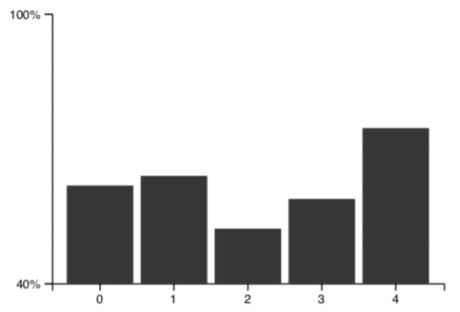
\includegraphics[width = 0.4\linewidth]{ExperienceTruncatingAxis-Bars-Correll2019.JPG} 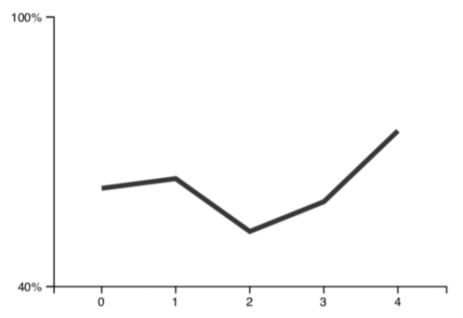
\includegraphics[width = 0.4\linewidth]{ExperienceTruncatingAxis-Lines-Correll2019.JPG}
\captionof*{figure}{\color{DarkSlateGray} {\textbf{Figure 1b:} Truncation serves to exaggerate effect sizes in  both line and bar charts. }}
\end{center}

\section*{Rule \#2: Modify the Framing Design}
Framing a graphic in a wide or tall format can also affect the perception of a phenomena, typically for time series.

\begin{center}\vspace{1cm}
            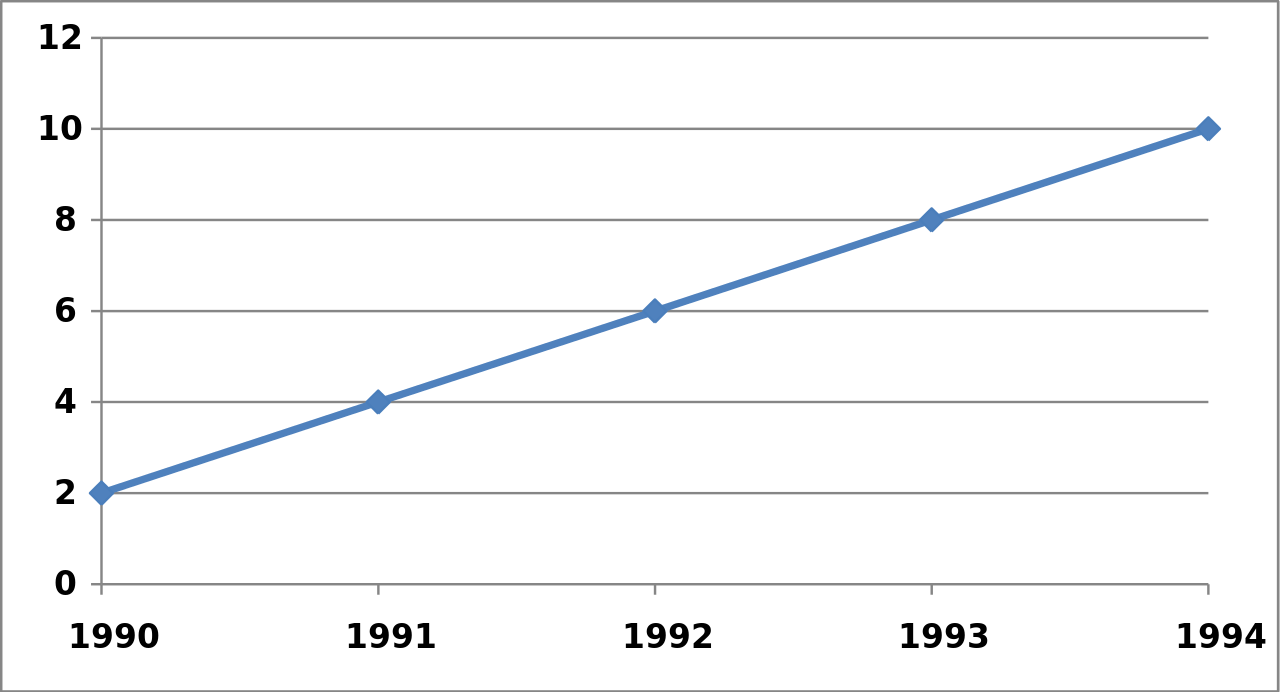
\includegraphics[width = 0.3\linewidth]{Line_graph1.png}
            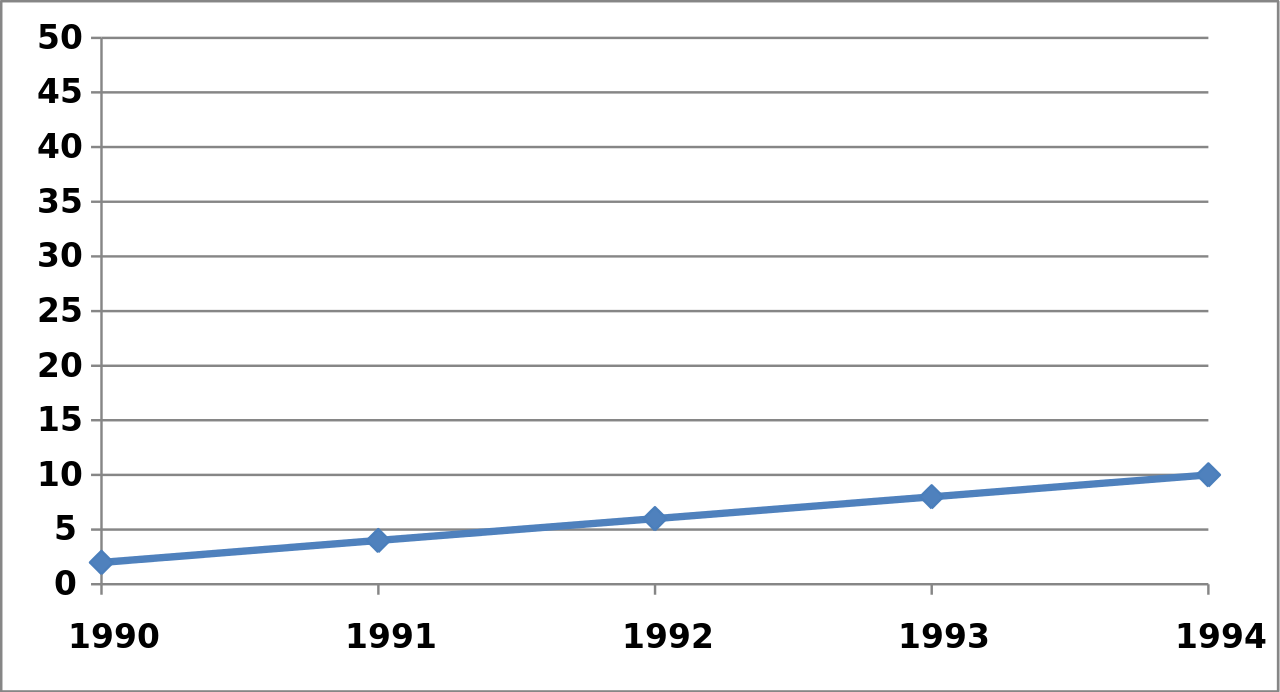
\includegraphics[width = 0.3\linewidth]{Line_graph2.png}
            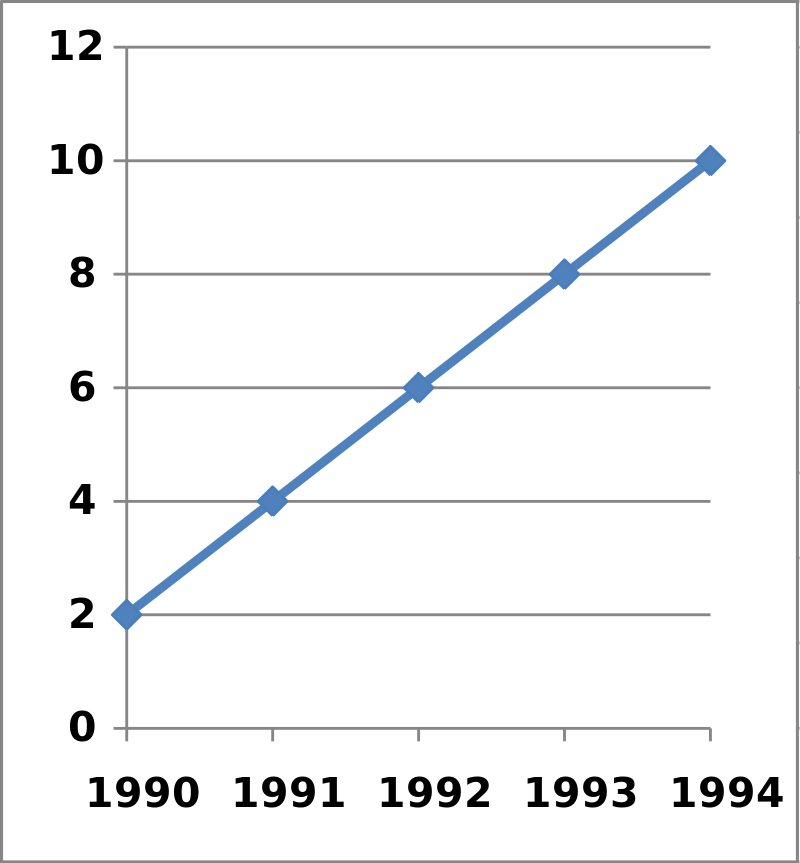
\includegraphics[width = 0.2\linewidth]{Line_graph1-3.png}\\
            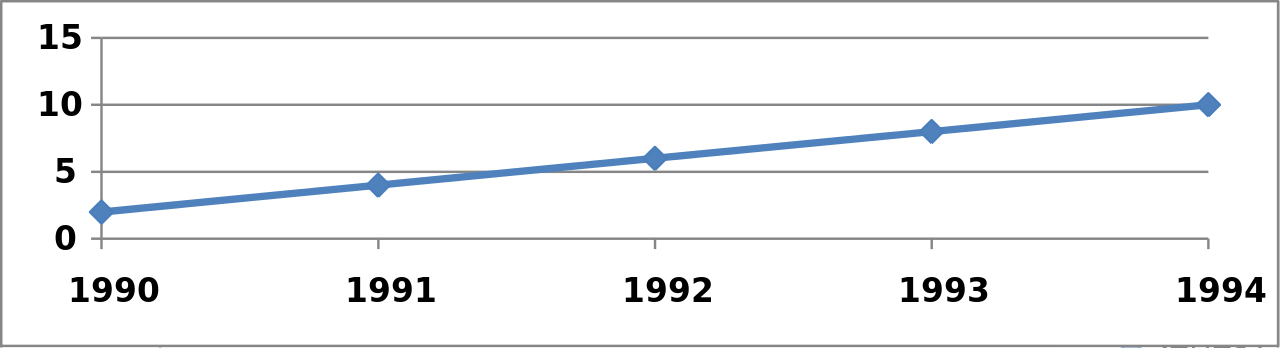
\includegraphics[width = 0.6\linewidth]{Line_graph1-4.png}
\captionof{figure}{\color{DarkSlateGray} {The perception of a time series increases is affected by the framing}}
\end{center}
But the framing, and space left around data points can subtly affect our perception of correlation  \cite{Cleveland1982}.
\begin{center}
 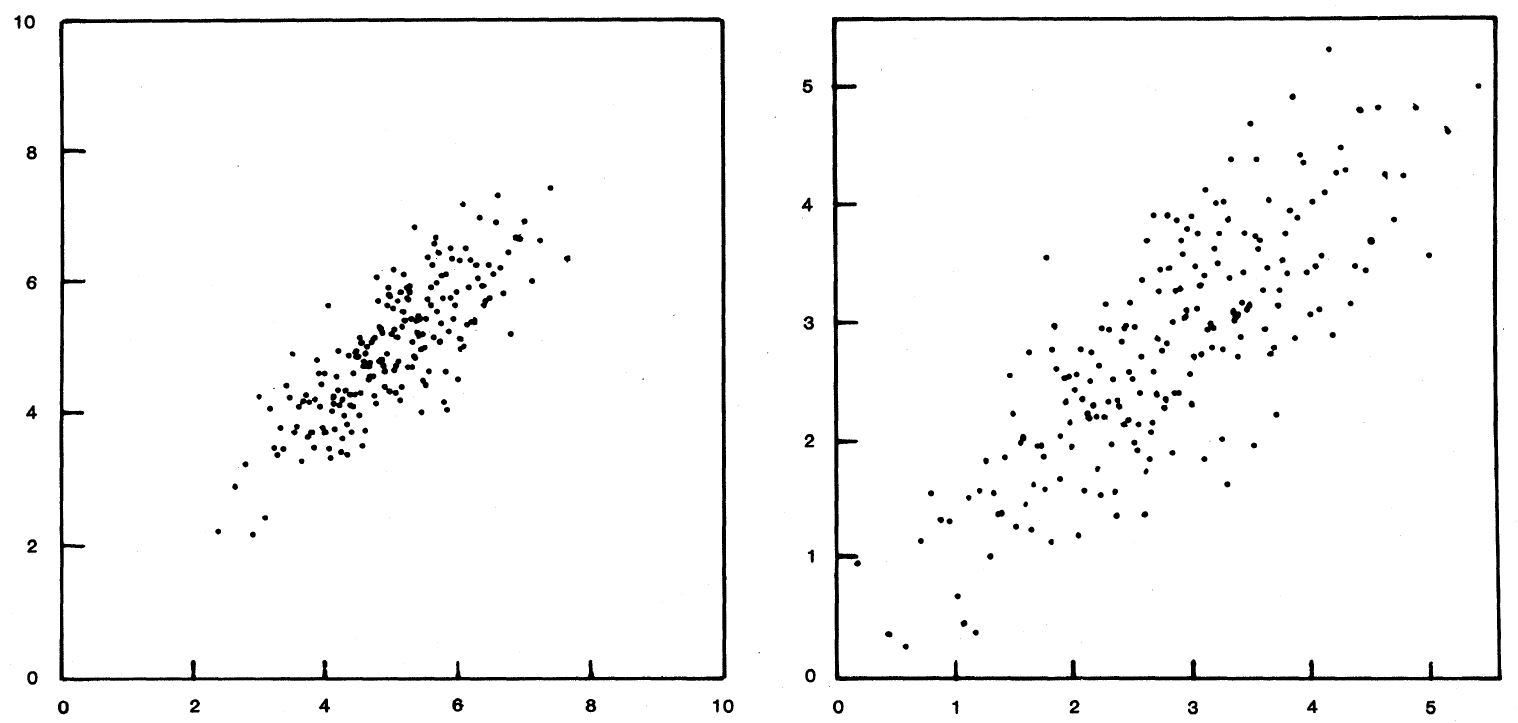
\includegraphics[width =0.6\linewidth]{ScalesScatterplotConcentrationCleveland.JPG}
 \captionof*{figure}{\color{DarkSlateGray} {\textbf{Figure 2b:} The correlation  between Xs and Ys is the same in the two data sets.  }}

\end{center}

\section*{Rule \#3: Use Double Axes}

Plotting two times series with different units on two axis (left and right) is a tempting practice that results in a spurious visual correlation. This has been well illustrated in \cite{muth2018} (see also \cite{Vigen2015}).
\begin{center}
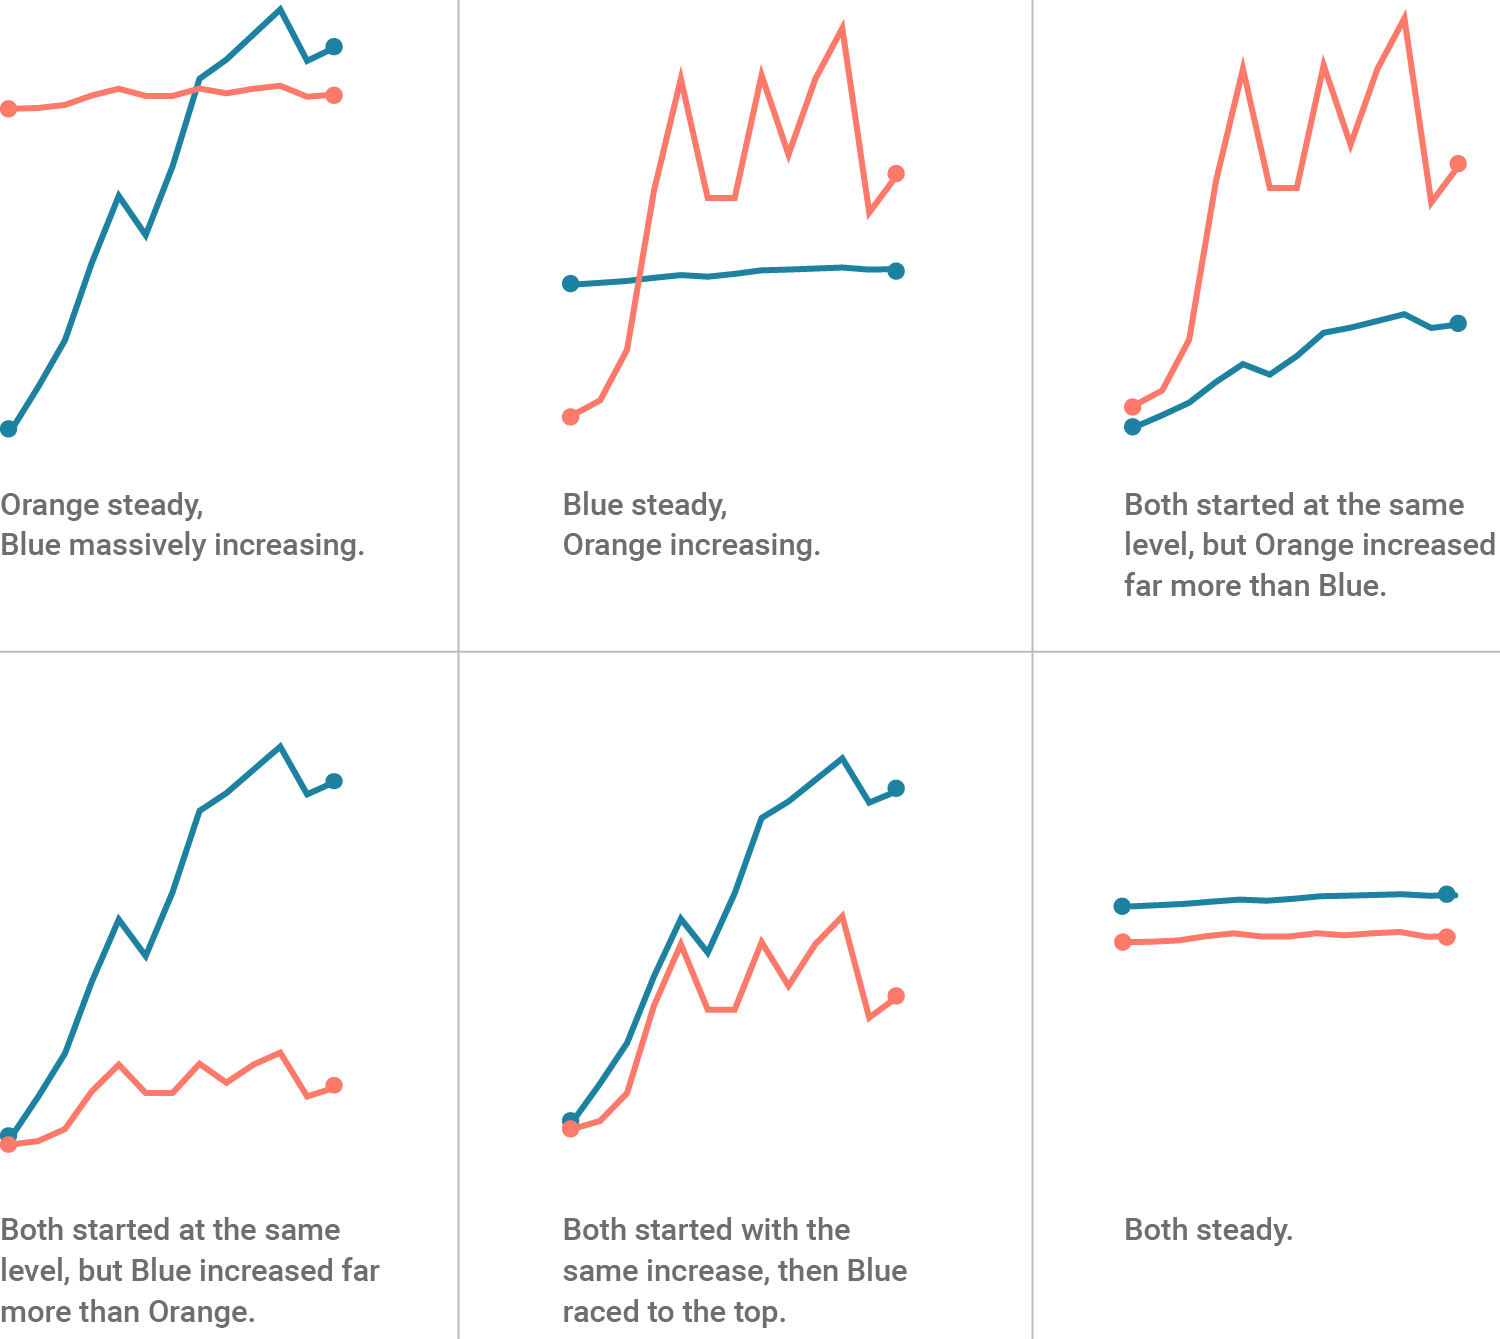
\includegraphics[width = 0.7\linewidth]{LCRost-dualaxisCrazy.png}
\captionof{figure}{\color{DarkSlateGray} {Playing with left and right axes (source: \cite{muth2018})}}
\end{center}


\textbf{ Cite \cite{isenberg_study_2011} HERE}


\section*{Rule \#4: Select Your Scope}
Cherry-picking the data through an (in)appropriate choice of the range in any time series, is alsovery misleading. This is particularly true for time serie and scatter plots but can also change the representation of maps when only a part of the world is selected as illustrated in \cite{bahoken2020}.

\begin{center}
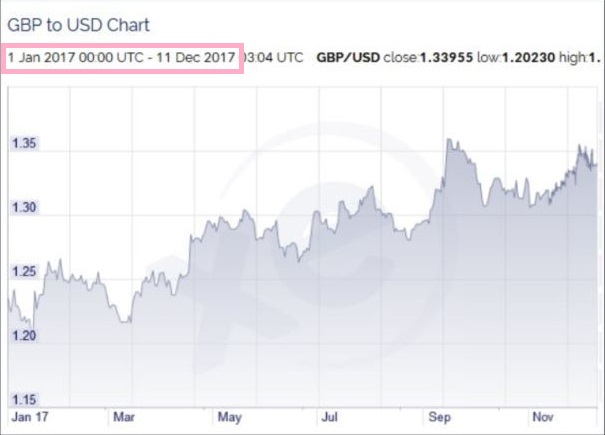
\includegraphics[width = 0.4\linewidth]{GBP-USDRate-Brexiters-Zoom.jpg} \hspace{0.5cm}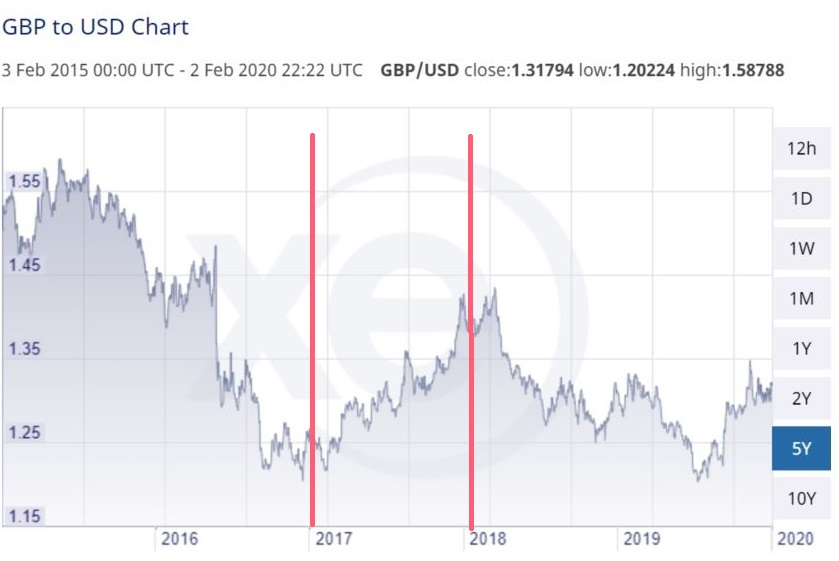
\includegraphics[width = 0.4\linewidth]{GBP-USDRate-5Y-Annotated.jpg}
\captionof{figure}{\color{DarkSlateGray} {A growing exchange rate (left) "picked" within a declining period (right)}}

\end{center}

\section*{Rule \#5: Use Several Pie Charts}
Pie charts are among the most popular and most used graphics although they are not suited for fair comparisons (\cite{Cleveland1984})
\begin{center}
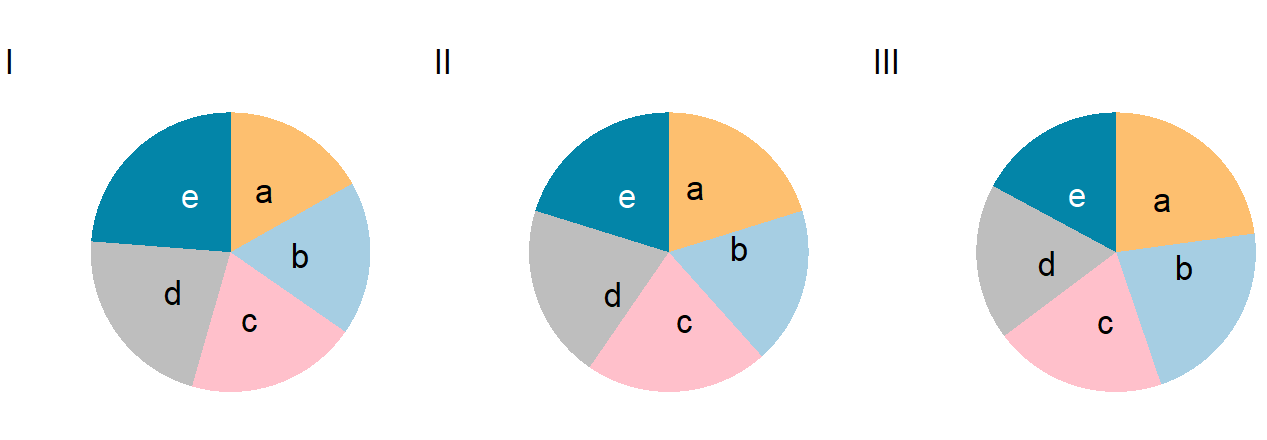
\includegraphics[width = 0.7\linewidth]{Compare3Pies.png}
\captionof{figure}{\color{DarkSlateGray} {Comparing pie charts can be a difficult visual test and should be avoided}}
\end{center}

\section*{Rule \#6: Use Areas}
Our perception of areas is very bad but area-based comparisons still flourishing in publication, in particular in statistical maps where buble maps are one of the most popular encoding (see rule \#10)

\begin{center}
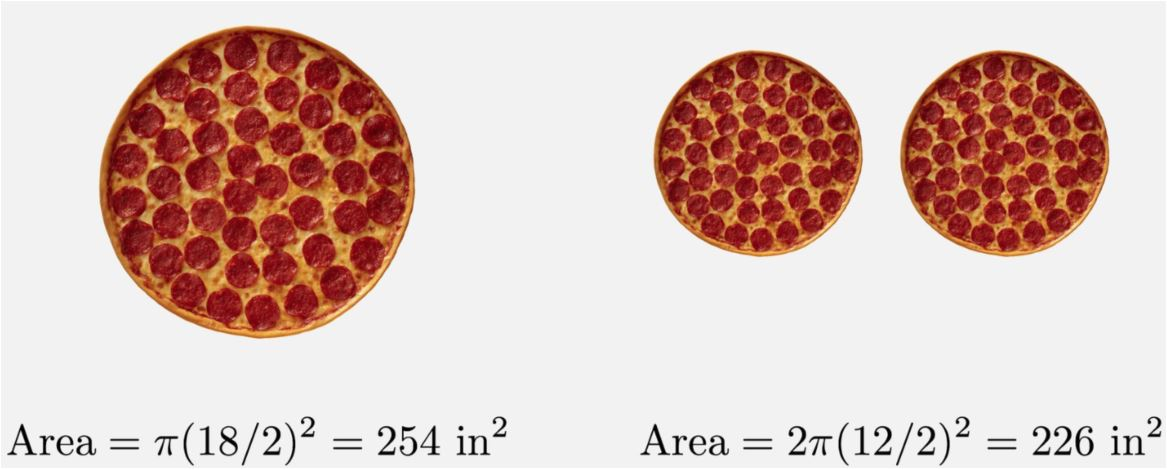
\includegraphics[width = 0.7\linewidth]{PizzaCircleslegend.jpg}
\captionof{figure}{\color{DarkSlateGray} {A simple exercise show that people think 2 pizzas are bigger than one }}

\end{center}


\section*{Rule \#7: Use unaligned bars}
Stacked bars are a good example of unaligned visual variables that are difficult to compare. In the example below, it is difficult to test whether the red category is steadily increasing or not.
\begin{center}
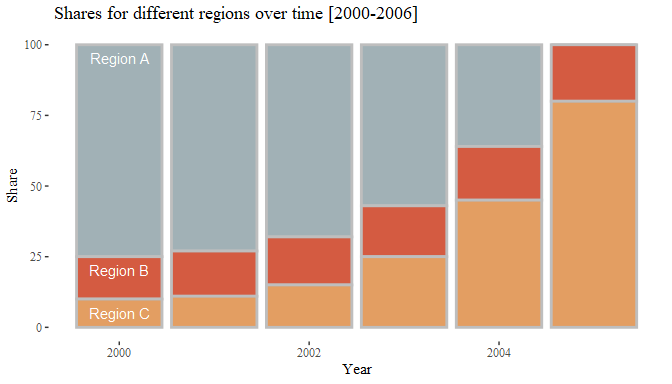
\includegraphics[width = 0.4\linewidth]{StackedBars-1.png} \hspace{0.2cm} vs \hspace{0.4cm}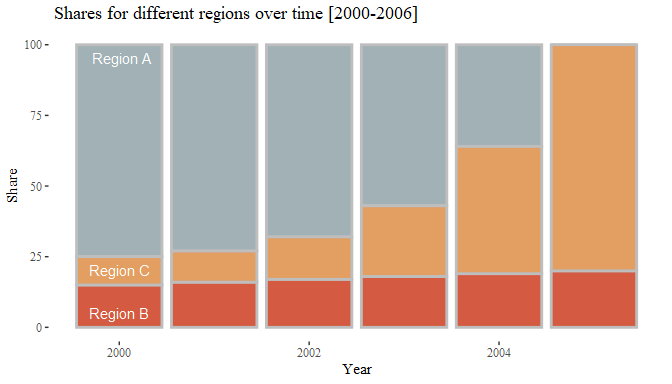
\includegraphics[width = 0.4\linewidth]{OrderedStakedBars-1.png}
\captionof{figure}{\color{DarkSlateGray} {In simple situations, ordering the categories may solve the problem }}
\end{center}


\section*{Rule \#8: Cross The Lines}
This is probably the most challenging as plotting several crossing lines is likely to produce a graphic where not clear pattern emerges as illustrated by  \cite{Schwabish2014} Alternative design using small multiples graphics, where only one line is highlighted while others are greyed for global reference, helps displaying clear information.
\begin{center}
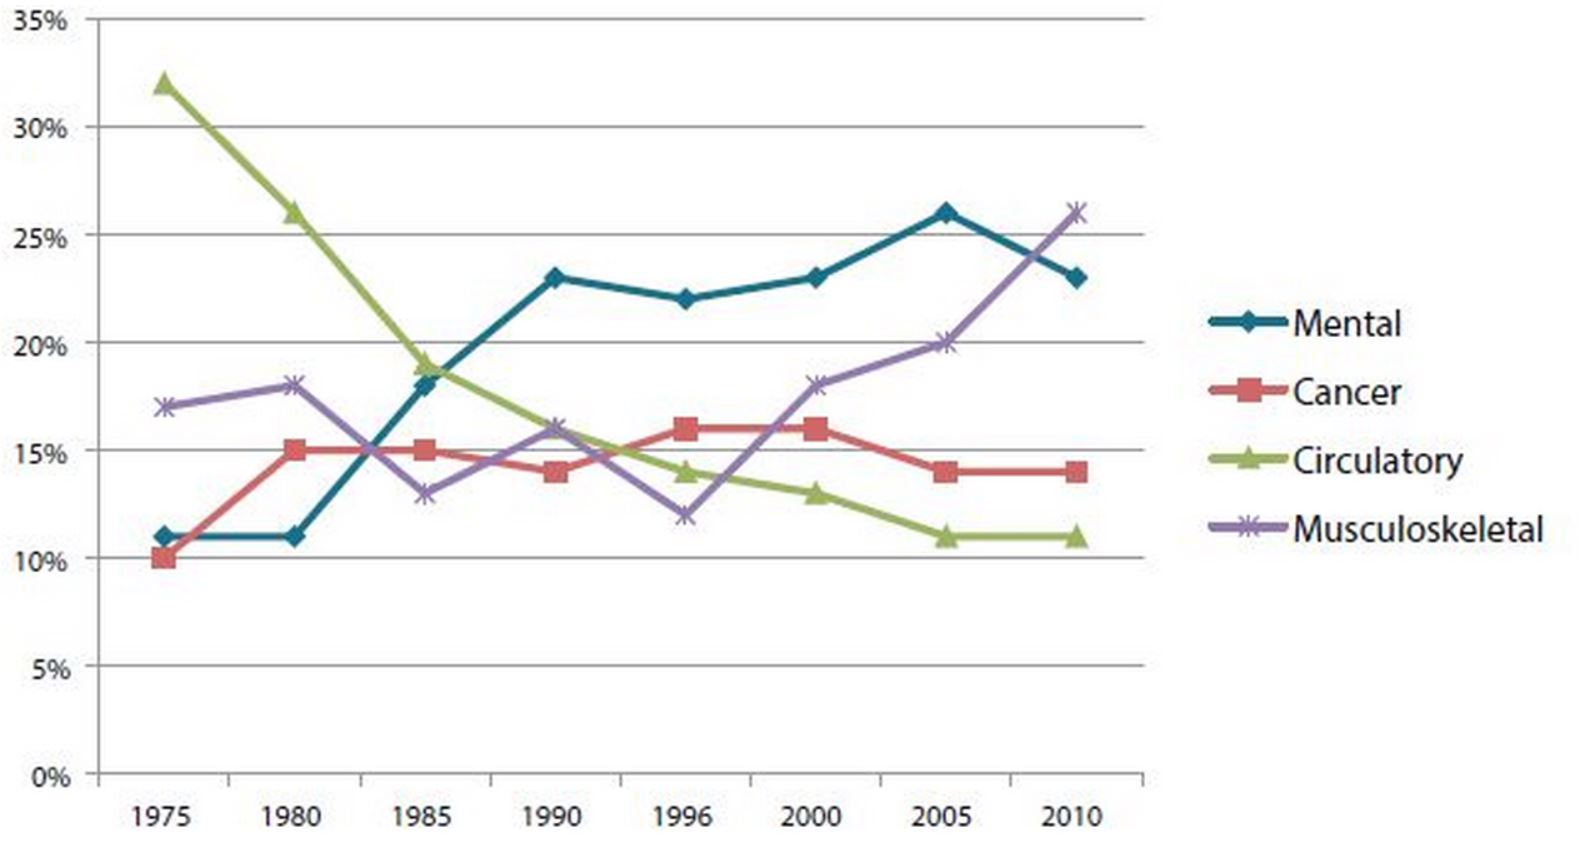
\includegraphics[width = 0.45\linewidth]{Spaghetti0.jpg} \hspace{0.2cm} vs \hspace{0.2cm}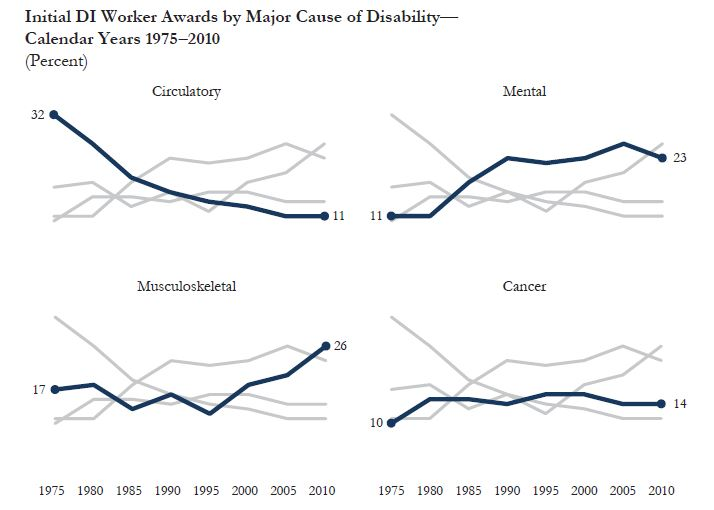
\includegraphics[width = 0.3\linewidth]{Spaghetti2.jpg}
\captionof{figure}{\color{DarkSlateGray} {In simple situations, ordering the categories may solve the problem }}

\end{center}

\section*{Rule \#9: Use Radar Plots}
Comparing individuals in many dimension is challenging, even when the sample in small. Using a data set of 4 individuals \cite{Bontemps2017} illustrated that the area representing the overall performance is highly dependant of the ordering of the axes. This undesirable feature is a major undocumented drawback of radar plots.
\begin{center}
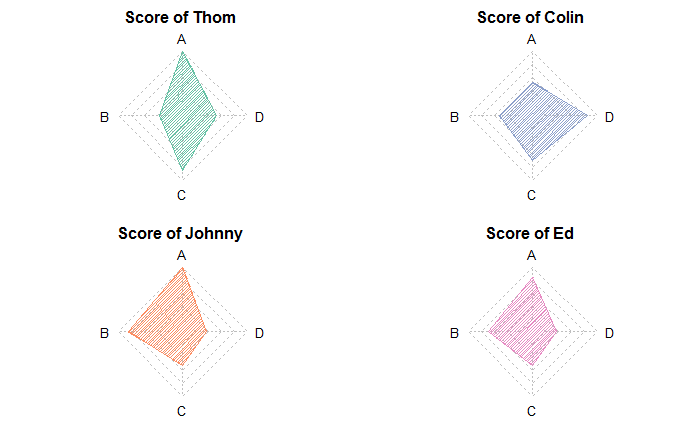
\includegraphics[width = 0.4\linewidth]{Radar1.png} \hspace{0.2cm} vs \hspace{0.2cm}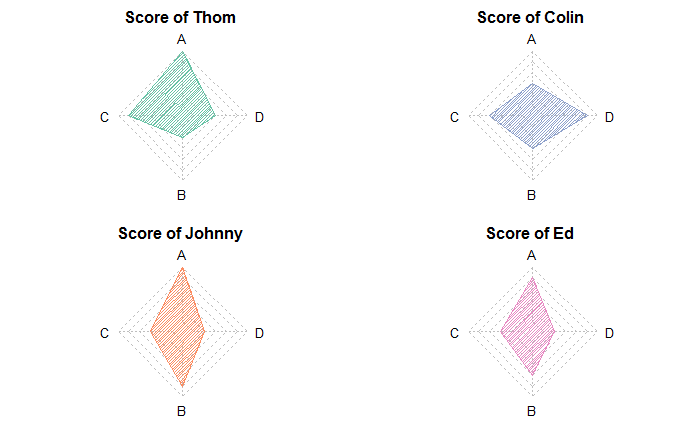
\includegraphics[width = 0.4\linewidth]{Radar2.png}
\captionof{figure}{\color{DarkSlateGray} {The order of the axes changes the areas  representing global  performance}}

\end{center}

\section*{Rule \#10: Use Maps}
Maps are probably the most complex graphical objects and are prone to many issues as documented by \cite{Monmonier1991} and others. Statistical maps use all the visual encoding described here, and thus concentrate all the problems hindering fair visual tests.

\begin{center}
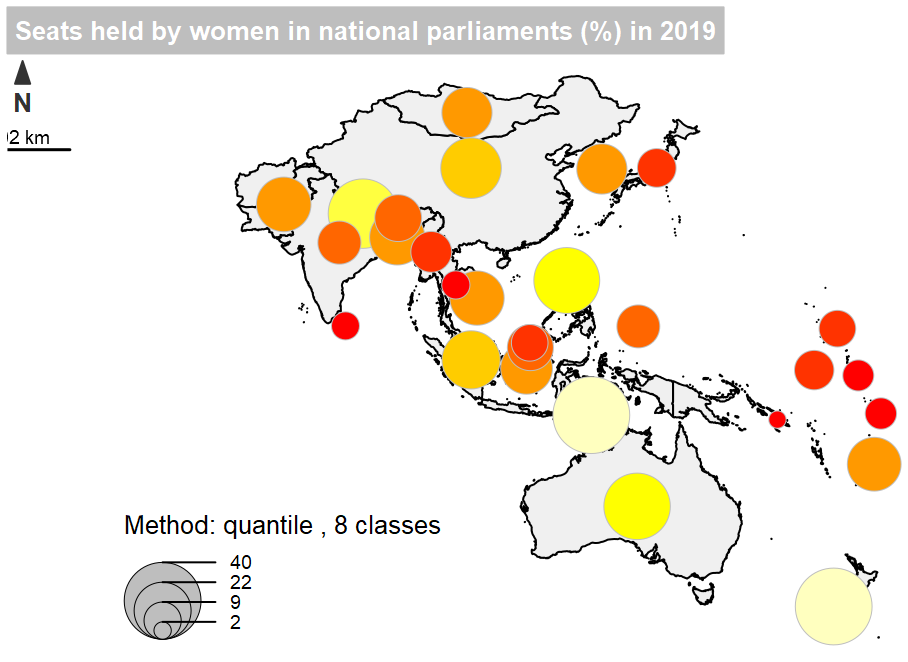
\includegraphics[width = 0.45\linewidth]{BubbleMapC.png} 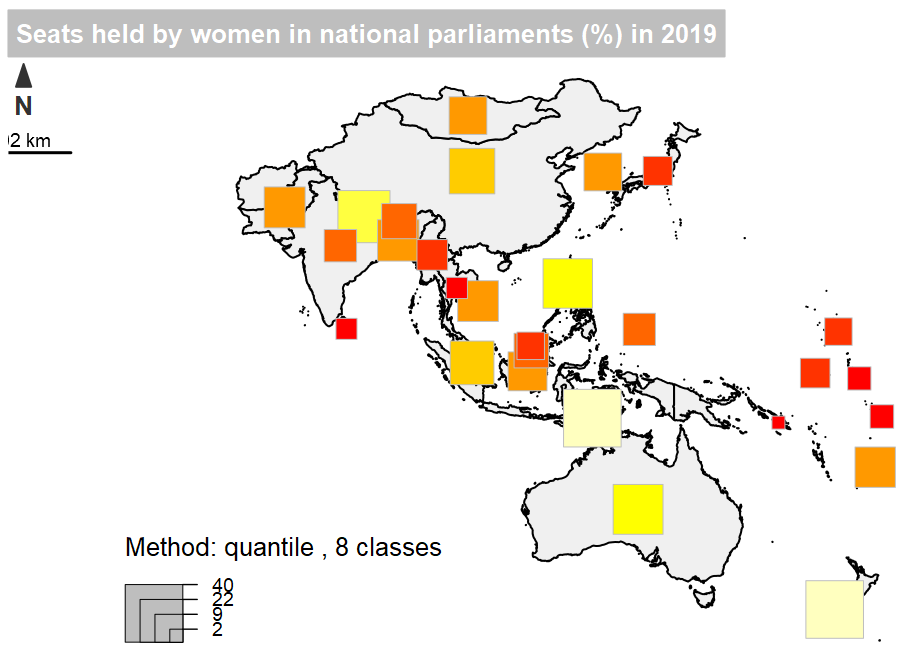
\includegraphics[width = 0.45\linewidth]{BubbleMapSquaresC.png} \\
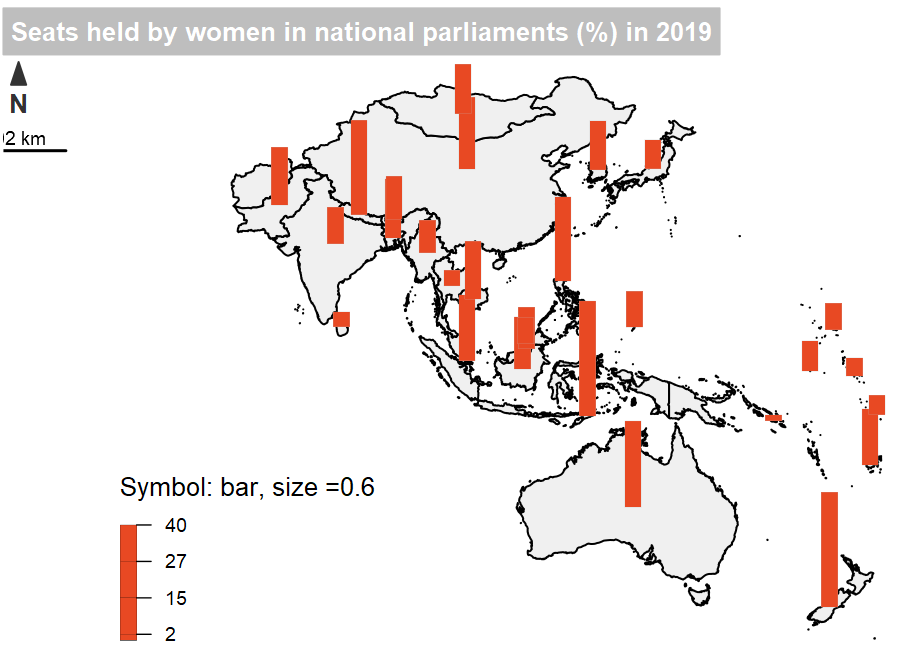
\includegraphics[width = 0.45\linewidth]{BubbleMapBarsC.png} 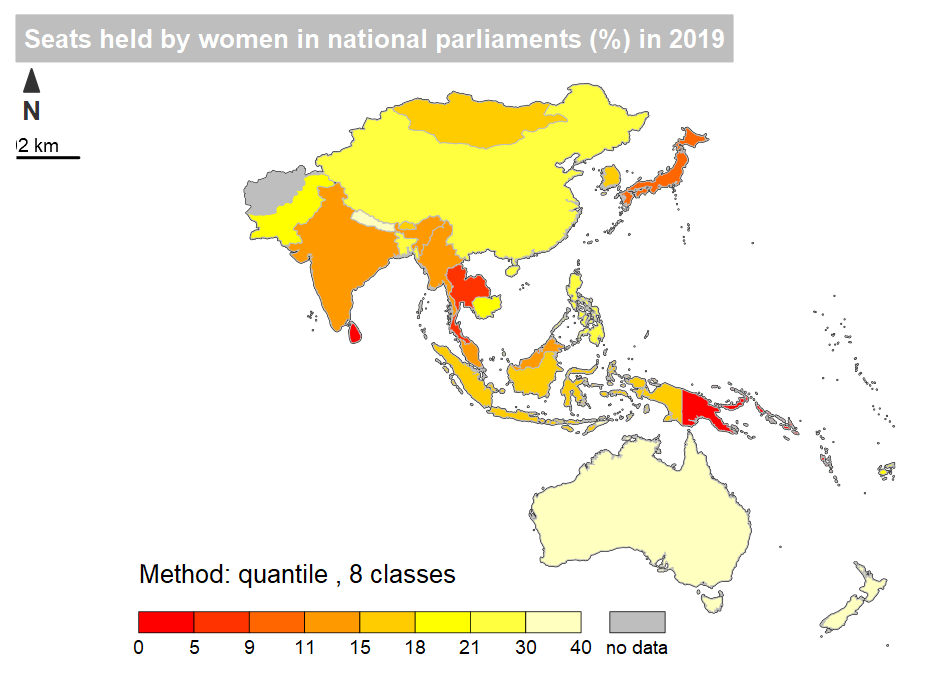
\includegraphics[width = 0.45\linewidth]{BubbleMapChoroplethC.png}
\captionof{figure}{\textcolor{DarkSlateGray}{4 ways of representing statistical information on a map, and many issues!}}
\end{center}



%----------------------------------------------------------------------------------------
%	CONCLUSIONS
%----------------------------------------------------------------------------------------



\section*{Conclusion}

Since the publication of \cite{Bertin1977}, a lot has been learned on the design of statistical information and on the use of data visualization as a visual language, with a clear semiology. Many publications have highlighted good practices for quite a long time (see the "old" \cite{Brinton1914}), but despite this abundant literature, very few articles have illustrated the dangers  of  easy-to-produce and popular  graphics. We should not let these useful visual tests be biased by software default settings, misconceived designs or uninformed statisticians.




%
%\nocite{*} % Print all references regardless of whether they were cited in the poster or not
%\bibliographystyle{plain} % Plain referencing style
\bibliographystyle{apalike}


% SHOULD USE THIS FOR IAOS !!
%\bibliographystyle{unsrtnat}  % <- Vancouver
%\bibliographystyle{authordate1_vp}
\bibliography{Visu, VisuSeminal, VisuOS}
%----------------------------------------------------------------------------------------
%	ACKNOWLEDGEMENTS
%----------------------------------------------------------------------------------------

%%\section*{Acknowledgements}
%%
%%This work was initiated a long time ago and find its roots in a series of lectures while the author was still at the Toulouse School of Economics and actively contributing to the non-profit organization Toulouse Dataviz.

%----------------------------------------------------------------------------------------

\end{document} 